\documentclass{standalone}

\usepackage{tikz-feynman}
\usepackage{tikz}

\usepackage{fontspec}
\setmainfont{Libertinus Serif}
\setsansfont{Libertinus Sans}
\usepackage[
  math-style=ISO,
  bold-style=ISO,
  sans-style=italic,
  nabla=upright,
  partial=upright,
]{unicode-math}
\setmathfont{Libertinus Math}

\tikzfeynmanset{compat=1.1.0}
\usetikzlibrary{decorations.pathreplacing}

\begin{document}
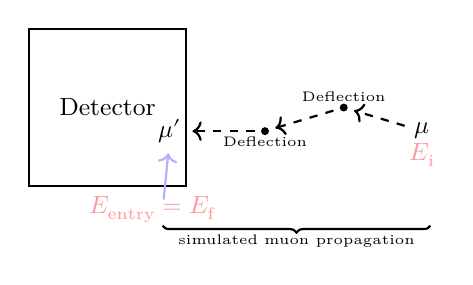
\begin{tikzpicture}[thick]
   % \tikzstyle{every node}=[font=\small]
 % \node (mu) at (-0.6,0) {$\mu$};
 % \node (x) at (1,0) {};
 % \node at (x) {$x$};
 % \node (mu_) at (2.5, 1) {}; 
 % \node at (mu_.east) {$\mu^\prime$};
 % \draw[thick, ->] (mu) -- (x);
 % \draw[thick, ->] (x) -- (mu_);
 % \draw[dashed] (x) -- (2.39, 0);
  % \filldraw[fill=green!20,draw=green!50!black] (1.1, 0) -- (1.3, 0) arc (1.3:0.5) -- cycle;
 % \draw (2,0) arc (0:33:1);
 % \node (theta) at (1.7, 0.25) {$\theta$};

	\node[rectangle,draw,minimum height=2cm, minimum width=2cm, font=\small] (r) at (0,0) {Detector};
	\node (x) at (0.8,-0.3) {\small $\mu^{\prime}$};
	\node (x1) at (2,-0.3) {};
	\node (x2) at (3,0) {};
	\node (x3) at (4,-0.3) {\small $\mu$};
%	\node at (x.south) {muon entry};
	\draw[dashed,->] (x1) -- (x);
	\draw[dashed, ->] (x2) -- (x1);
	\draw[dashed, ->] (x3) -- (x2);
	\filldraw (x1) circle (1pt);
	\filldraw (x2) circle (1pt);
	\node[font=\tiny] at (x1.south) {Deflection};
	\node[font=\tiny] at (x2.north) {Deflection};
	\node (xx) at (0.7, -1.3) {};
	\draw[thick, ->, draw=blue!30] (xx) -- (x);
	\node[font=\small, text=red!40] at (xx.west) {$E_{\mathrm{entry}} = E_{\mathrm{f}}$};
	\node[font=\small, text=red!40] at (4,-0.6) {$E_{\mathrm{i}}$};
	\draw[decorate,decoration = {brace, mirror, raise=1.2cm}] (0.7,-0.3) -- (4.1,-0.3) node[midway,yshift=-1.4cm] {\tiny simulated muon propagation};



%     \node at (0,0) {\includegraphics[width=1\textwidth]{atlas.jpg}};
%     \node (TRT) at (5,-3) {TRT Tracker};
%     \node (PD) at (2.5,-3) {Pixel Detector};
%     \node (SM) at (0,-3.04) {Solenoid Magnet};
%     \node (EM) at (5,3.5) {EM calorimeter};
%     \node (HC) at (1,3.5) {Hadronic calorimeter};
%     \node (MS) at (-3,3.46) {Muon spectrometer};
%     \draw [thick,decoration={brace,mirror,raise=0.2cm},decorate] (SM.west) -- (TRT.east)
% node [pos=0.5,anchor=north,yshift=-0.3cm] {Inner detector};
%     \draw[thick,->] (TRT.north) -- (1.5,0.1);
%     \draw[thick,->] (PD.north) -- (1.1,0.2);
%     \draw[thick,->] (SM.north) -- (0.8,0.2);
%     \draw[thick,->] (EM.south) -- (2,0.5);
%     \draw[thick,->] (EM.south) -- (1.5,0.5);
%     \draw[thick,->] (HC.south) -- (1.2,0.7);
%     \draw[thick,->] (MS.south) -- (-3.3,1.4);
%     \draw[thick,->] (MS.south) -- (0.5,2);


    % \filldraw[draw=blue,fill=blue!20] (0,0) rectangle (4,3.15);
    % \filldraw[draw=red,fill=red!20] (0.5,0.5) rectangle (2.5,2.5);
    % \draw[draw=none, pattern=north west lines, pattern color=black!50] (2.015,0.515) rectangle (2.485,2.485);
    % \draw [dashed] (2,3.15) -- (2,0);
    % \node at (1, 2.75) {$\mathsf{\textit{N}_{\mathrm{L}}^{\,\mathrm{r}}}$};
    % \node at (3, 2.79) {$\mathsf{\textit{N}_{\mathrm{L}}^{\,\mathrm{f}}}$};
    % \node at (1.3,1.5) {$\mathsf{\textit{N}_{\mathrm{T}}^{\,\mathrm{r}}}$};
    % \node at (2.25,1.54) {$\mathsf{\textit{N}_{\mathrm{T}}^{\,\mathrm{f}}}$};
    % \draw[->, >=stealth, thick] (1.2,2.75) ..controls (1.7,2.3) and (1.5,2).. (1.3,1.7);
    % \node at (1.3,2.15) {$\epsilon^{\mathrm{r}}$};
    % \draw[->, >=stealth, thick] (2.9,2.6) ..controls (2.9,2.4) and (3.0,2.0).. (2.45,1.5);
    % \node at (3.05,2.2) {$\epsilon^{\mathrm{f}}$};
    % \node at (0.5, 0.25) {\textcolor{blue}{loose}};
    % \node at (1,0.75) {\textcolor{red}{tight}};
\end{tikzpicture}
\end{document}
